\pdfoutput=1
\pdfminorversion=7

\documentclass[aspectratio=169]{beamer}
% \documentclass{beamer}

\usetheme{metropolis}

% Intel palette
\definecolor{DarkBlue}{HTML}{003C71}
\definecolor{Blue}{HTML}{0071C5}
\definecolor{LightBlue}{HTML}{00AEEF}
\definecolor{Gray}{HTML}{B1BABF}
\definecolor{Orange}{HTML}{FFA300}
\definecolor{Red}{HTML}{FC4C02}
\definecolor{White}{HTML}{FFFFFF}
\setbeamercolor{alerted text}{fg=Blue}
\setbeamercolor{frametitle}{bg=Blue}
\setbeamercolor{palette primary}{fg=White, bg=Blue}

\setbeamerfont{footnote}{size=\fontsize{3pt}{3pt}\selectfont}
\setbeamertemplate{frame numbering}[none]

\usepackage{xspace}
\newcommand{\themename}{\textbf{\textsc{metropolis}}\xspace}

\title{The Path to DPDK Speeds for AF\_XDP}
\author{Magnus Karlsson, Björn Töpel}
\date{magnus.karlsson@intel.com, bjorn.topel@intel.com}
\institute{Linux Plumbers Conference, Vancouver, 2018}
\titlegraphic{\hfill
\includegraphics[width=2cm]{intel-logo.pdf}} 

\newcommand{\srcsize}{\@setfontsize{\srcsize}{3pt}{3pt}}

\begin{document}
  \maketitle

  \begin{frame}{Legal Disclaimer}
  \tiny
  \begin{itemize}
  \item Intel technologies may require enabled hardware, specific software, or services activation. Check with your system manufacturer or retailer.
  \item No computer system can be absolutely secure.
  \item Tests document performance of components on a particular test, in specific systems. Differences in hardware, software, or configuration will affect actual performance. Consult other sources of information to evaluate performance as you consider your purchase. For more complete information about performance and benchmark results, visit www.intel.com/benchmarks.
  \item Cost reduction scenarios described are intended as examples of how a given Intel- based product, in the specified circumstances and configurations, may affect future costs and provide cost savings. Circumstances will vary. Intel does not guarantee any costs or cost reduction.
  \item All information provided here is subject to change without notice. Contact your Intel representative to obtain the latest Intel product specifications and roadmaps.
  \item No license (express or implied, by estoppel or otherwise) to any intellectual property rights is granted by this document.
  \item Intel does not control or audit third-party benchmark data or the web sites referenced in this document. You should visit the referenced web site and confirm whether referenced data are accurate.
  \item Intel, the Intel logo, and other Intel product and solution names in this presentation are trademarks of Intel.
  \item Other names and brands may be claimed as the property of others.
  \item \copyright 2018 Intel Corporation.
  \end{itemize}
  \end{frame}

  \begin{frame}{XDP 101}
    \centering\resizebox{!}{.95\textheight}{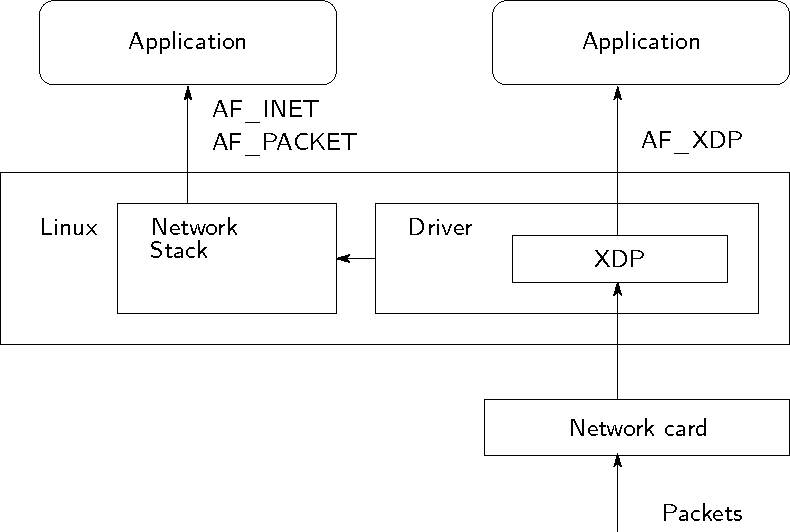
\includegraphics{xdp-new.pdf}}
  \end{frame}

  \begin{frame}{AF\_XDP 101}
    \begin{itemize}
    \item Ingress
      \begin{itemize}
      \item userspace XDP packet sink
      \item {\tt XDP\_REDIRECT} to socket via {\tt XSKMAP}
      \end{itemize}
    \item Egress
      \begin{itemize}
      \item no XDP program
      \end{itemize}
    \item Register userspace packet buffer memory to kernel (UMEM)
    \item Pass packet buffer ownership via descriptor rings
    \end{itemize}
  \end{frame}

  \begin{frame}{AF\_XDP 101}
    \centering\resizebox{\textwidth}{!}{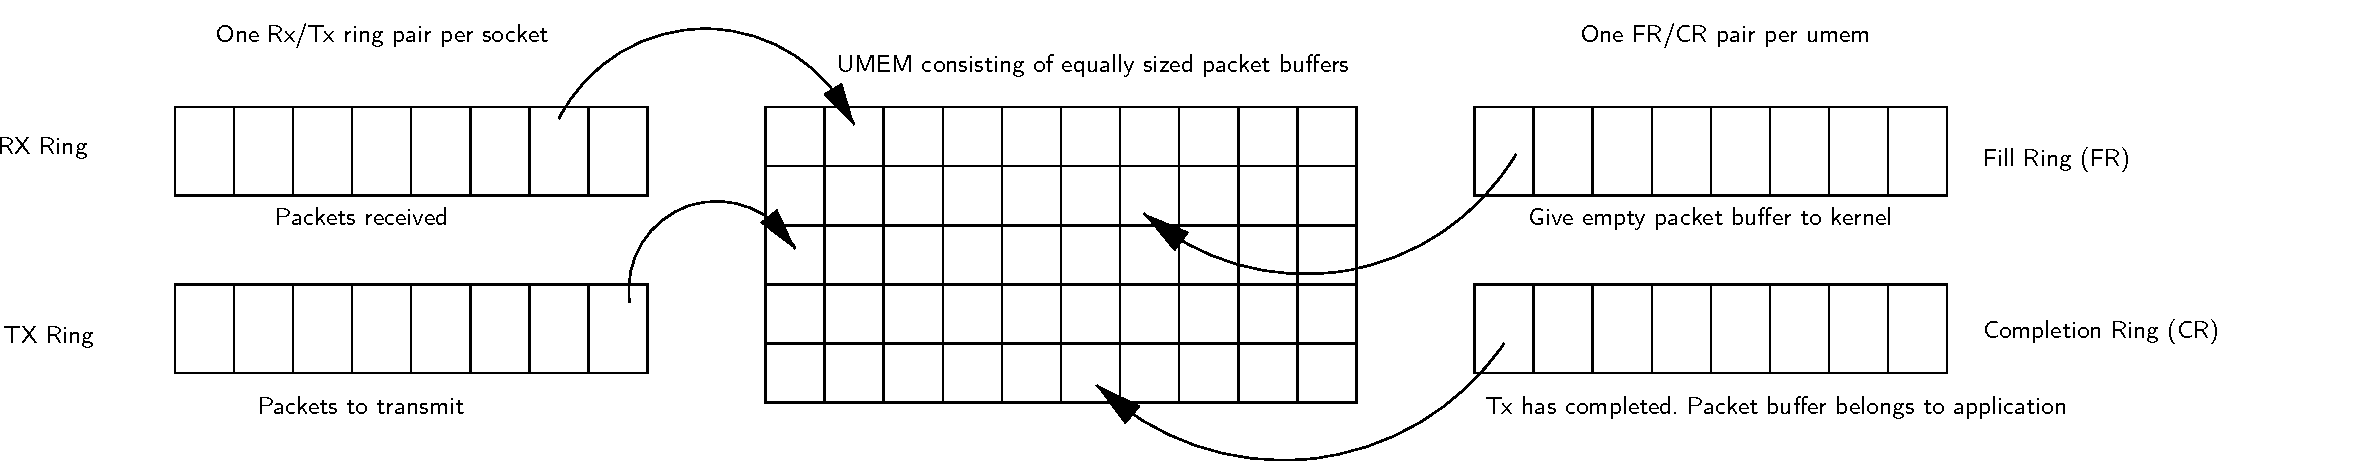
\includegraphics{queues_and_umem-new.pdf}}
    \begin{itemize}
    \item Fill ring (to kernel) / Rx ring (from kernel)
    \item Tx ring (to kernel) / Completion ring (from kernel)
    \item copy mode (DMA to/from kernel allocated frames, copy data to user)
    \item zero-copy mode (DMA to/from user allocated frames)
    \end{itemize}
  \end{frame}

  \begin{frame}{Baseline and optimization strategy}
      \begin{itemize}
      \item Baseline
      \begin{itemize}
      \item Linux 4.20
      \item 64B @ \textasciitilde15-22 Mpps
      \end{itemize}

      \item Strategy
      \begin{itemize}
        \item do less (instructions)
        \item talk less (coherency traffic)
        \item do more at the same time (batching, i\$)
        \item Land of Spectres: fewer retpolines, fewer retpolines,
          fewer repolines
      \end{itemize}
      \end{itemize}
  \end{frame}

  \begin{frame}{Experimental Setup}
  \begin{itemize}
  \item Broadwell E5-2660 @ 2.7GHz
  \item 2 cores used for run-to-completion benchmarks
  \item 1 core used for busy-poll benchmarks
  \item 2 i40e 40GBit/s netdevs, 2 AF\_XDP sockets
  \item Ixia load generator blasting at full 40 Gbit/s per NIC
  \end{itemize}
  \end{frame}

  \begin{frame}{Ingress}
      \begin{itemize}
        \item {\tt XDP\_ATTACH} and {\tt bpf\_xsk\_redirect}, attach
          at-most one socket per netdev queue, load built-in XDP
          program, 2-level hierarchy
        \item remove indirect call, {\tt bpf\_prog\_run\_xdp}
        \item remove indirect call, XDP actions switch-statement ($>=5
          \implies$ jump table)
        \item driver optimizations (batching, code restructure)
        \item {\tt bpf\_prog\_run\_xdp}, {\tt xdp\_do\_redirect} and
          {\tt xdp\_do\_flush\_map}: per-CPU {\tt struct
            bpf\_redirect\_info} + {\tt struct xdp\_buff} + {\tt
            struct xdp\_rxq\_info} vs explicit, stack-based context
      \end{itemize}
  \end{frame}

  \begin{frame}{Ingress, results\footnotemark[1], data not touched}
    \centering\resizebox{!}{.85\textheight}{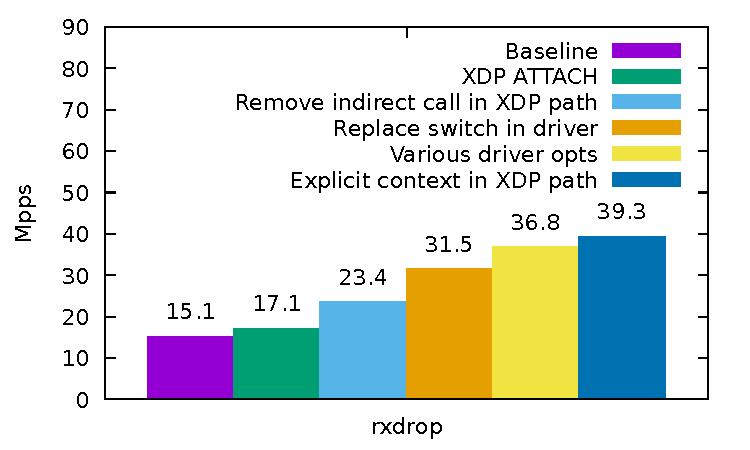
\includegraphics{results_rx.pdf}}
      \footnotetext[1]{
      Results have bee nestimated based on internal Intel analysis and
      are provided for informational purposes only. Any difference in
      system hardware or software design or configuration may affect
      actual performance. Software and workloads used in performance
      tests may have been optimized for performance only on Intel
      microprocessors. Performance tests, such as SYSmark and
      MobileMark, are measured using specific computer systems,
      components, software, operations and functions. Any change to
      any of those factors may cause the results to vary. You should
      consult other information and performance tests to assist you in
      fully evaluating your contemplated purchases, including the
      performance of that product when combined with other
      products. For more information go
      to http://www.intel.com/performance/datacenter.}
  \end{frame}

  \begin{frame}{Egress}
  \begin{columns}[T,onlytextwidth]
    \column{0.5\textwidth}
    \begin{itemize}
    \item Tx performance capped per HW queue $\implies$ multiple Tx
      sockets per UMEM
    \item Larger/more batching, larger descriptor rings
    \item Dedicated AF\_XDP HW Tx queues
    \item In-order complettion, {\tt setsockopt} {\tt XDP\_INORDER\_COMPLETION}
    \end{itemize}
    \column{0.5\textwidth}      
    \centering\resizebox{\textwidth}{!}{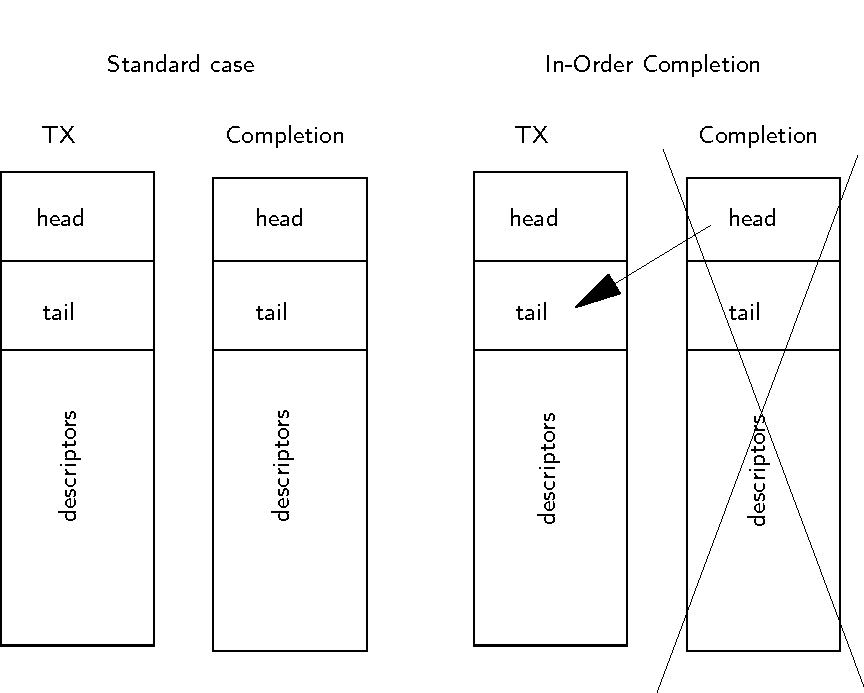
\includegraphics{in_order-new.pdf}}
    \end{columns}
  \end{frame}

  \begin{frame}{Egress, results\footnotemark[1], data not touched}
    \centering\resizebox{!}{.85\textheight}{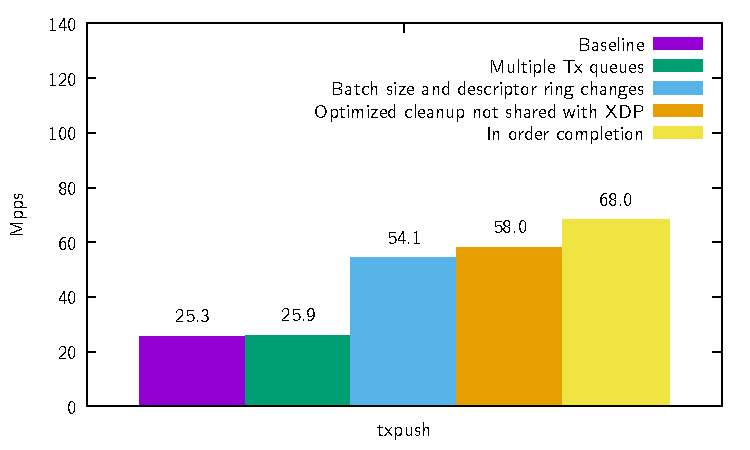
\includegraphics{results_tx.pdf}}
      \footnotetext[1]{
      Results have bee nestimated based on internal Intel analysis and
      are provided for informational purposes only. Any difference in
      system hardware or software design or configuration may affect
      actual performance. Software and workloads used in performance
      tests may have been optimized for performance only on Intel
      microprocessors. Performance tests, such as SYSmark and
      MobileMark, are measured using specific computer systems,
      components, software, operations and functions. Any change to
      any of those factors may cause the results to vary. You should
      consult other information and performance tests to assist you in
      fully evaluating your contemplated purchases, including the
      performance of that product when combined with other
      products. For more information go
      to http://www.intel.com/performance/datacenter.}
  \end{frame}

  \begin{frame}{Busy poll() vs run-to-completion}
    \centering\resizebox{!}{0.9\textheight}{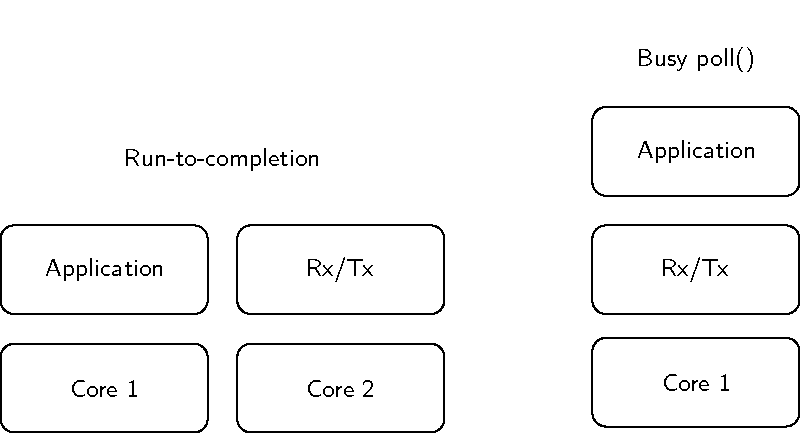
\includegraphics{two_vs_one_core-new.pdf}}
  \end{frame}

  \begin{frame}{Busy poll() vs run-to-completion, results\footnotemark[1]}
    \centering\resizebox{!}{.85\textheight}{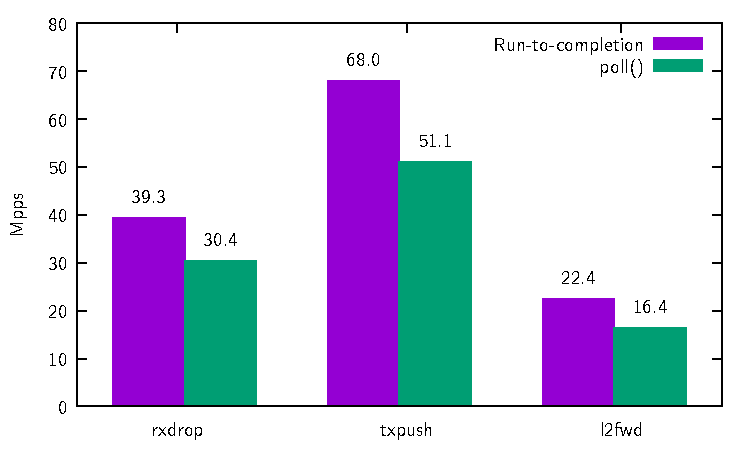
\includegraphics{results_poll.pdf}}
      \footnotetext[1]{
      Results have bee nestimated based on internal Intel analysis and
      are provided for informational purposes only. Any difference in
      system hardware or software design or configuration may affect
      actual performance. Software and workloads used in performance
      tests may have been optimized for performance only on Intel
      microprocessors. Performance tests, such as SYSmark and
      MobileMark, are measured using specific computer systems,
      components, software, operations and functions. Any change to
      any of those factors may cause the results to vary. You should
      consult other information and performance tests to assist you in
      fully evaluating your contemplated purchases, including the
      performance of that product when combined with other
      products. For more information go
      to http://www.intel.com/performance/datacenter.}
  \end{frame}

  \begin{frame}{Comparison with DPDK}
    \begin{itemize}
      \item Userspace, vectorized drivers
      \item ``Learning from the DPDK''
        \url{http://vger.kernel.org/netconf2018_files/StephenHemminger_netconf2018.pdf}
    \end{itemize}
  \end{frame}

  \begin{frame}{Comparison with DPDK, results\footnotemark[1]}
    \centering\resizebox{!}{.85\textheight}{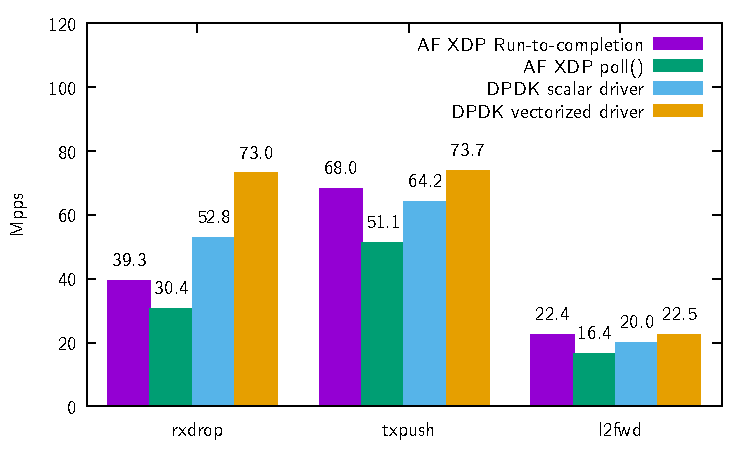
\includegraphics{results_dpdk.pdf}}
      \footnotetext[1]{
      Results have bee nestimated based on internal Intel analysis and
      are provided for informational purposes only. Any difference in
      system hardware or software design or configuration may affect
      actual performance. Software and workloads used in performance
      tests may have been optimized for performance only on Intel
      microprocessors. Performance tests, such as SYSmark and
      MobileMark, are measured using specific computer systems,
      components, software, operations and functions. Any change to
      any of those factors may cause the results to vary. You should
      consult other information and performance tests to assist you in
      fully evaluating your contemplated purchases, including the
      performance of that product when combined with other
      products. For more information go
      to http://www.intel.com/performance/datacenter.}
  \end{frame}

  \begin{frame}{Next steps}
    Upstream!
    \begin{itemize}
      \item XDP: switch-statement
      \item Rx/Tx: drivers
      \item Rx: {\tt XDP\_ATTTACH} and {\tt bpf\_xsk\_redirect}
      \item libbpf AF\_XDP support
      \item Tx: multiple Tx sockets per UMEM
      \item selftest, samples
    \end{itemize}    
  \end{frame}

  \begin{frame}{Future work}
    \begin{itemize}
    \item hugepage support, less fill ring traffic ({\tt
      get\_user\_pages})
    \item fd.io/VPP work vectors (i\$, explicit batching in function calls)
    \item ``XDP first'' drivers 
    \item collaborate/share code with RDMA (e.g. {\tt
      get\_user\_pages})
    \item Type-writer model (currently not planned)
    \end{itemize}
  \end{frame}
  % TODO Talk about built-in plus copy for tcpdump based on AF_XDP?

  \begin{frame}{TL;DR}
  \begin{itemize}
  \item Rx 15.1 to 39.3 Mpps (260\%)
  \item Tx 25.3 to 68.0 Mpps (269\%)
  \item Busy poll() promising
  \item DPDK still faster for ``notouch'', but AF\_XDP on par when data is touched
  \item drivers need to change when skb is not the only consumer
  \end{itemize}
  \end{frame}

  \begin{frame}{Thanks!}
  \begin{columns}[T,onlytextwidth]
    \column{0.5\textwidth}
    \begin{itemize}
    \item Ilias Apalodimas
    \item Daniel Borkmann
    \item Jesper Dangaard Brouer
    \item Willem De Bruijn
    \item Eric Dumazet
    \item Alexander Duyck
    \item Mykyta Iziumtsev
    \item Jakub Kicinski
    \item Song Liu
    \end{itemize}
    
    \column{0.5\textwidth}
    \begin{itemize}
    \item David S. Miller
    \item Pavel Odintsov
    \item Sridhar Samudrala
    \item Yonghong Song
    \item Alexei Starovoitov
    \item William Tu
    \item Anil Vasudevan
    \item Jingjing Wu
    \item Qi Zhang
    \end{itemize}
  \end{columns}
  \end{frame}

  \begin{frame}[standout]
    Questions?
    \resizebox{\textwidth}{!}{
\includegraphics{af_xdp_vit.pdf}}
  \end{frame}

\end{document}
